\documentclass[10pt,landscape]{article}
\usepackage{amsmath}
\usepackage{dsfont}
\usepackage{multicol}
\usepackage{clrscode3e}
\usepackage[landscape]{geometry}

\usepackage{pgf}
\usepackage{tikz}
\usetikzlibrary{arrows,automata}


% Tiny margins
\geometry{top=1cm,left=1cm,right=1cm,bottom=1cm}

% Turn off header and footer
\pagestyle{empty}

% Redefine section commands to use less space
\makeatletter
\renewcommand{\section}{\@startsection{section}{1}{0mm}%
                                {-1ex plus -.5ex minus -.2ex}%
                                {0.5ex plus .2ex}%x
                                {\normalfont\large\bfseries}}
\renewcommand{\subsection}{\@startsection{subsection}{2}{0mm}%
                                {-1explus -.5ex minus -.2ex}%
                                {0.5ex plus .2ex}%
                                {\normalfont\normalsize\bfseries}}
\renewcommand{\subsubsection}{\@startsection{subsubsection}{3}{0mm}%
                                {-1ex plus -.5ex minus -.2ex}%
                                {1ex plus .2ex}%
                                {\normalfont\small\bfseries}}
\makeatother

% Don't print section numbers
\setcounter{secnumdepth}{0}

% Set paragraph parameters.
\setlength{\parindent}{0pt}
\setlength{\parskip}{2pt plus 0.5ex}

% More macros:
\let\oldforall\forall
\renewcommand{\forall}{\hspace{2pt} \oldforall \hspace{1pt}}

\newcommand{\definition}[1]{\textbf{#1}\hspace{2pt}}

% -----------------------------------------------------------------------

\begin{document}

\raggedright
\footnotesize
\begin{multicols}{3}


% multicol parameters
% These lengths are set only within the two main columns
%\setlength{\columnseprule}{0.25pt}
\setlength{\premulticols}{1pt}
\setlength{\postmulticols}{1pt}
\setlength{\multicolsep}{1pt}
\setlength{\columnsep}{2pt}

\begin{center}
     \Large{\textbf{6.046 Exam 2 Cheat Sheet}} \\
\end{center}

\section{Early lecture trivia}

\definition{Matrix Multiplication} Two $n \times n$ matrices can be multiplied in $O(n^{2.376})$ time.

%------------------------------------

\section{Lecture 8: Greedy Algorithms and MST}

\definition{Kruskal's Algorithm} Pick the lowest-weight edge such that no cycles are formed at each step.

\definition{Prim's Algorithm} Pick a starting vertex and grow from there, on any vertex yet spanned.

%------------------------------------

\section{Lecture 9: Gradient Descent}

placeholder

%------------------------------------

\section{Lecture 10: Maxflow-Mincut}

\definition{Value of flow} $|f| = \sum\limits_{v \in V} f(s, v) - \sum\limits_{v \in V} f(v,s)$

\definition{Max-Flow Problem} Given a network $G = (V, E, s, t, c)$, find a flow of maximum value.

\definition{Augmenting Path} A path from $s$ to $t$, such that not all edges on the path are at capacity.

\definition{Ford-Fulkerson Algorithm}

\begin{enumerate}
\item $f = 0$
\item While there is an augmenting path $p$, send max possible flow along $p$.
\item Return $f$.
\end{enumerate}

This is $O(E)$ per augmentation, and if all capacities are integers, the whole algorithm terminates in $O(Ef)$. F-F with BFS has worst-case runtime of $O(VE^2)$.

\definition{Min-Cut Problem} Given a network $G = (V, E, s, t, c)$, find a cut of minimum capacity.

All $s-t$ cuts have the same capacity because of conservation of flow.

\definition{Maxflow-Mincut Theorem} The value of the max flow is equal to the capacity of the min-cut for any network.
%------------------------------------

\section{Lecture 11: Vertex Cover and Matching}

\definition{Vertex Cover}  A set of vertices in a graph that touch all edges in a graph.

For instance:

\begin{center}
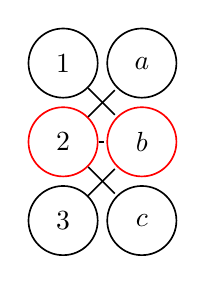
\begin{tikzpicture}[>=stealth',shorten >=1pt,auto,node distance=1cm,
                    semithick]

  \node[state]         (one)                    {1};
  \node[state]         (two) [below of=one, draw=red] {2};
  \node[state]         (thr) [below of=two] {3};
  \node[state]         (A) [right of=one] {$a$};
  \node[state]         (B) [below of=A, draw=red]       {$b$};
  \node[state]         (C) [below of=B]       {$c$};

  \path (one) edge              node {} (B)
        (two) edge           node {} (A)
            edge              node {} (B)
            edge              node {} (C)
        (thr) edge              node {} (B);
\end{tikzpicture}
\end{center}

\underline{Goal}: Given an undirected graph, find a vertex cover of minimum size.

This problem is NP-Complete. We know that these are all solvable within $O(e^x)$ time, but not that they don't have a polynomial time algorithm solution.

\definition{Bipartite Graphs} $G = (L \cup R, E \subseteq L \times R)$ for disjoint sets of vertices $L$ and $R$.

A helpful way to think about this is to sandwich the bipartite graph between a start and end node (source and sink). Furthermore, we change the undirected graph to make it directed, such that each edge is directed from $L$ to $R$, with infinite capacities (a la Maxflow).

\begin{center}
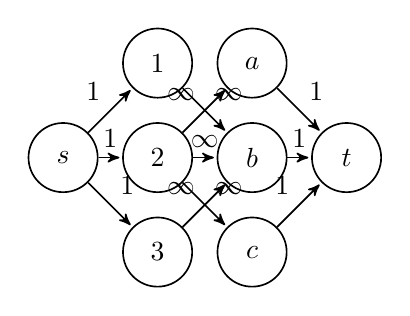
\begin{tikzpicture}[->, >=stealth',shorten >=1pt,auto,node distance=1.2cm,
                    semithick]
  \node[state]         (one)                    {1};
  \node[state]         (two) [below of=one] {2};
  \node[state]         (thr) [below of=two] {3};
  \node[state]         (A) [right of=one] {$a$};
  \node[state]         (B) [below of=A]       {$b$};
  \node[state]         (C) [below of=B]       {$c$};
  \node[state]         (S) [left of=two] {$s$};
  \node[state]         (T) [right of=B] {$t$};

  \path (one) edge              node {$\infty$} (B)
        (two) edge           node {$\infty$} (A)
            edge              node {$\infty$} (B)
            edge              node {$\infty$} (C)
        (thr) edge              node {$\infty$} (B)
        (S) edge node {1} (one)
              edge node {1} (two)
              edge node {1} (thr)
        (A) edge node {1} (T)
        (B) edge node {1} (T)
        (C) edge node {1} (T);
\end{tikzpicture}
\end{center}

The flow of $G'$ is the size of the Minimum VC of $G$.

\definition{Matching}: A set of edges of a graph that share no endpoints.

Let the below graph be $G$. A matching is highlighted.

\begin{center}
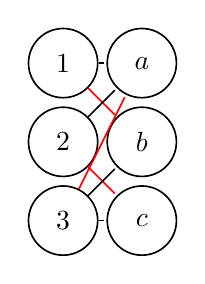
\begin{tikzpicture}[>=stealth',shorten >=1pt,auto,node distance=1cm,
                    semithick]

  \node[state]         (one)                    {1};
  \node[state]         (two) [below of=one] {2};
  \node[state]         (thr) [below of=two] {3};
  \node[state]         (A) [right of=one] {$a$};
  \node[state]         (B) [below of=A]       {$b$};
  \node[state]         (C) [below of=B]       {$c$};

  \path (one) edge              node {} (A)
                    edge [draw=red] node {} (B)
        (two) edge           node {} (A)
            edge [draw=red] node {} (C)
        (thr) edge [draw=red] node {} (A)
        edge              node {} (B)
        edge              node {} (C);
\end{tikzpicture}
\end{center}

As before, set up an $s$ and a $t$ node. This time, set all capacities to 1, rather than $\infty$. We call the below graph $G''$.

\begin{center}
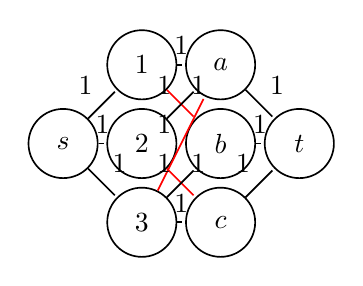
\begin{tikzpicture}[>=stealth',shorten >=1pt,auto,node distance=1cm,
                    semithick]

  \node[state]         (one)                    {1};
  \node[state]         (two) [below of=one] {2};
  \node[state]         (thr) [below of=two] {3};
  \node[state]         (A) [right of=one] {$a$};
  \node[state]         (B) [below of=A]       {$b$};
  \node[state]         (C) [below of=B]       {$c$};
  \node[state]         (S) [left of=two] {$s$};
  \node[state]         (T) [right of=B] {$t$};

  \path (one) edge              node {1} (A)
                    edge [draw=red] node {1} (B)
        (two) edge           node {1} (A)
            edge [draw=red] node {1} (C)
        (thr) edge [draw=red] node {1} (A)
        edge              node {1} (B)
        edge              node {1} (C)
        (S) edge node {1} (one)
              edge node {1} (two)
              edge node {1} (thr)
        (A) edge node {1} (T)
        (B) edge node {1} (T)
        (C) edge node {1} (T);
\end{tikzpicture}
\end{center}

\underline{Goal}: Given a graph, find maximum matching $|M| \leq \frac{|V|}{2}$.

\definition{Konig's Theorem (1931)}: In bipartite graphs, the size of the maximum matching is the same as the size of the minimum vertex cover.

\definition{Alternating Path}: A path in a bipartite graph where every second edge is used in the matching.

\definition{Augmenting path}: An alternating path where both the first and the last vertices are unmatched.

If you flip what you consider matched and unmatched in an augmenting path, then you get a matching of bigger size. Not sure what I meant by this when I wrote it, but I'm keeping it in the cheat sheet for the exam.

%------------------------------------

\section{Lecture 12: Linear Programming}

\definition{Linear Program} Minimize or maximize a linear objective function subject to linear inequalities.

\definition{Standard LP Form} $\max \vec{c} \cdot \vec{x}$ subject to constraints $A \vec{x} \leq \vec{b}$ and $\vec{x} \geq 0$.

% Note: you don't actually say how to do these algorithms.

\definition{Simplex Algorithm} $\vec{x}$ walks from vertex to vertex in direction of $\vec{c}$. Worst-case exponential.

\definition{Interior-Point Method} $\vec{x}$ moves inside polytope vaguely $\vec{c}$-wards. $O(n^{3.5} \cdot L^2)$, where $n$ is the number of variables and $L$ is the number of bits required to describe the constraints to the LP.

\definition{Strong LP Duality} A maximization problem in standard from can be transformed into the \textbf{dual} as follows: $\min \vec{b} \cdot \vec{y}$ s.t. $A^{\top} \cdot \vec{y} \geq \vec{c}$ and $\vec{y} \geq 0$.

The dual has the same solution to the optimization problem as the other LP, but no other points overlap.

\definition{Weak LP Duality} $\vec{c} \cdot \vec{x} \leq OPT_{\max} \leq OPT_{\min} \leq \vec{b} \cdot \vec{y}$

%------------------------------------

\section{Lecture 13: Game Theory and the MinMax Theorem}

\definition{Stable Strategy} A set of choices for a given game from which no agent increases expected value by diverging from.

\definition{Nash Equilibrium} A stable state for a given game.

\definition{Nash's Theorem} ``In every finite game, (finite \# players and finite \# strategies for each), $\exists$ a collection of randomized strategies (one per player) s.t. no player can improve their expected payout by unilaterally changing their strategy."

You can prove the probabilities for a Nash equilibrium by assigning variable probabilities ($x_1, x_2$, etc.) for one player, and setting it up as a linear program with $\mathds{E}[option] \geq z$, for each option, and the sum of the probabilities is 1.

By strong LP duality, the solutions to each of those LPs are the opposite of one another ($val_{P1} = -val_{P2}$), in a Nash Equilibrium.

%Wait but what is the MinMax Theorem?

%------------------------------------

\section{Lecture 14: Dynamic Programming}

\definition{Memoizing} Implement recursive algorithm using look-up table. If the entry is null, it hasn't been solved before.

\definition{Iterating} Subproblems to be solved in an order which never requires the solving of subproblems that haven't been solved before. For instance, solving problems for all leaves and then working up the tree.

\definition{Catalan Numbers} The number of binary trees with $n$ nodes is the $n^{th}$ Catalan number $C(n) = \frac{1}{n+1} \binom{2n}{n} \approx \frac{4^n}{n^{3/4} \sqrt{\pi}}$

% Include the BST optimization problem here if time.

%------------------------------------

\section{Lecture 15: All-Pairs Shortest Path}

\definition{Single-Source Shortest Path (SSSP)} Given a directed graph $G(V,E)$, vertex $s \in V$, and edge weights $w: E \to \mathds{R}$, find $S(s,v)$, the shortest-weighted path from $s$ to $v \in V$, for all $v$.

\begin{tabular}{lll}
Algorithm & Time & Conditions \\ \hline
BFS & $O(V + E)$ & $w(e) = 1 \forall e \in E$ \\
Dijkstra & $O(E + V \log V)$ & $w(e) \geq 0 \forall e \in E$ \\
Bellman-Ford & $O(VE)$ & general \\
Toposort + BF & $O(V + E)$ & acyclic graph
\end{tabular}

\definition{All-Pairs Shortest Path} given $G(V,E, w)$, find $S(u,v) \forall u,v \in V$. There's another general algorithm for this specific problem that runs in $O(VE + V^2 \log V)$.

\definition{Floyd-Warshall Algorithm}

\begin{codebox}
\li $C \gets w(u, v)$
\li \For $k \gets 1 \twodots n$
\li \>\For $u \in V$
\li \>\>\For $v \in V$
\li \>\>\>\If $c_{uv} > c_{uk} + c_{kv}$: \Comment Relaxation
\li \>\>\>\> $c_{uv} \gets c_{uk} + c_{k_v}$
\end{codebox}

\definition{Johnson's Algorithm} Better than Floyd-Warshall for sparse graphs.

\begin{enumerate}
\item Find function $h: V \to \mathds{R}$ such that $w_h (u, v) = w(u,v) + h(u) - h(v) \geq 0 \forall u,v \in V$, or determine that a negative-weight cycle exists.
\item Run Dijkstra's algorithm on $(V, E, w_h)$, for every source vertex to get $S_h(u, v) \forall u,v \in V$.
\item $S(u,v) = S_h(u,v) + h(u) - h(v)$
\end{enumerate}

You find $h$ by solving a system of difference constraints (yay LPs!) for$h(v) - h(u) \leq w(u,v) \forall u,v \in V$.

%------------------------------------

\section{Lecture 16: NP-Completeness}

\definition{Optimization Problem} Find the best-case solution to the problem. Ex for MST: Find the cheapest spanning tree.
\definition{Search Problem} Find a solution that satisfies some search constraint. Ex for MST: given $G = (V, E, w)$, and a \underline{budget} $L$, find a  spanning tree of cost $\leq L$ (or report that none exists).
\definition{Decision Problem} Does a solution exist, given constraints? Ex for MST: Given $G$, budget $L$, is there a spanning tree of cost $\leq L$?

For any given algorithm, decision is easier than search is ``easier" than optimization, since you can solve search given optimization, and decision given search. So it's best to write an algorithm for optimization, and to prove hardness for decision.

\definition{Polynomial-time (P)} A decision problem $\Pi$ is in P if there is an algorithm $A$ with running time $|x|^c$ for some constant c such that $A(x)$ outputs the right answer (yes/no).

\definition{Non-deterministic polynomial time (NP)}. These are problems that can be \underline{verified} in polynomial time. Given a solution yes/no to the decision problem, and a polynomial length certificate $C$ that this is the right answer, there exists a polynomial time verification algorithm $V$ such that $V(x,c) = \text{yes} \Leftrightarrow x $ is a yes instance.

\definition{Reductions} Create a mapping between an unknown problem $\Pi_1$ and a known problem $\Pi_2$ whose runtime is known. If there is such a reduction, we say $\Pi_1 \leq_P \Pi_2$ if that reduction takes $P$ time to run.


\end{multicols}
\end{document}
